\documentclass[10pt, a4paper]{article}
\usepackage{fontawesome5}

% ---- PACKAGES ----
\usepackage[T1]{fontenc}
\usepackage[utf8]{inputenc}
\usepackage{times}
\usepackage[a4paper, top=1.8cm, bottom=1.8cm, left=2cm, right=2cm]{geometry}
\usepackage{xcolor}
\usepackage{titlesec}
\usepackage{enumitem}
\usepackage{hyperref}
\usepackage{tabularx}
\usepackage{array}
\usepackage{booktabs}
\usepackage{microtype}
\usepackage{parskip}
\usepackage{graphicx}
\usepackage{wrapfig}
\usepackage{ifthen}

% ---- COLORS ----
\definecolor{accentblue}{RGB}{47, 84, 150}   % Deep academic blue
\definecolor{lightgray}{RGB}{240, 240, 240}
\definecolor{darkgray}{RGB}{80, 80, 80}
\definecolor{medgray}{RGB}{120, 120, 120}

% ---- HYPERLINKS ----
\hypersetup{
  colorlinks=true,
  urlcolor=accentblue,
  linkcolor=accentblue,
  pdfborder={0 0 0}
}

% ---- NO PAGE NUMBER ----
\pagestyle{empty}

% ---- SECTION STYLE (Wandercraft-inspired: colored title + full-width rule) ----
\titleformat{\section}
  {\large\bfseries\color{accentblue}}
  {}{0em}{}
  [\vspace{-12pt}\textcolor{accentblue}{\rule{\linewidth}{0.8pt}}\vspace{2pt}]

\titlespacing*{\section}{0pt}{10pt}{4pt}

% ---- SUBSECTION: job/degree title ----
\titleformat{\subsection}[runin]
  {\normalsize\bfseries}
  {}{0em}{}[]
\titlespacing*{\subsection}{0pt}{5pt}{3pt}

% ---- LIST SETTINGS ----
\setlist[itemize]{leftmargin=1.4em, topsep=2pt, itemsep=1pt, parsep=0pt}
\renewcommand{\labelitemi}{\textbullet}

% ---- CUSTOM COMMANDS ----
% Entry: {Title}{Date}{Institution/Location}{bullets}
\newcommand{\cventry}[4]{%
  \noindent
  \begin{tabularx}{\linewidth}{@{}Xr@{}}
    {\fontsize{11.5}{12.5}\selectfont\textbf{#1}} & \textcolor{medgray}{#2}
  \end{tabularx}\\[0pt]
  \noindent{\textit{\textcolor{darkgray}{#3}}}
  \vspace{-4pt}
  \ifx&#4&\else
    \begin{itemize}#4\end{itemize}
  \fi
  \vspace{3pt}
}

% Publication entry
\newcommand{\pubentry}[1]{%
  \noindent\hangindent=1em\hangafter=1 #1\par\vspace{3pt}
}

% ====================================================
\begin{document}
% ====================================================

% ---- HEADER ----
\begin{minipage}[t]{0.72\linewidth}
  \vspace{0pt}
  {\LARGE\bfseries THOMAS LAVIGNE, PhD}\\[4pt]
  {\normalsize\textcolor{darkgray}{Post-Doctoral Researcher | Biomechanics \& Poromechanics}}\\[6pt]
  \textcolor{medgray}{%
    \faMapMarker\ 22 Esplanade Jacques Chirac, Suresnes, 92150, France\\[2pt]
    \faMobile\ +33 (0)7 50 28 93 48 \quad|\quad
    \faEnvelope\ \href{mailto:lavignethomas@hotmail.fr}{lavignethomas@hotmail.fr}\\[2pt]
    \faGlobe\ \href{https://th0maslavigne.github.io}{th0maslavigne.github.io} \quad|\quad
    \faOrcid\ ORCID: \href{https://orcid.org/0000-0003-2690-3542}{0000-0003-2690-3542}
  }
\end{minipage}%
\hfill
\begin{minipage}[t]{0.24\linewidth}
  \vspace{0pt}
  \raggedleft
  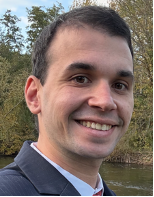
\includegraphics[width=2.6cm]{profile_pic.png}
\end{minipage}

\section*{PROFESSIONAL SUMMARY}
Computational biomechanics researcher specializing in the poromechanical and multiscale modeling of soft biological tissues. 
Awarded a Dual Doctoral Degree (cotutelle Université du Luxembourg / ENSAM Paris) focused on developing a physics-based, hierarchical porous media framework to understand human skin micro-circulation and pressure ulcer aetiology. 
Recognized for bridging complex theoretical developments, \textit{in vivo} experimental campaigns, and high-performance numerical implementation. Dedicated to Open Science and reproducibility, having developed open-source simulation tutorials and a Python package (FEniCSx). 
Described by the PhD defense jury as an exceptional scientist positioned to become a ``reference in this emerging field."

% ---- EDUCATION ----
\section{EDUCATION}

\cventry{Co-tutelle PhD in Engineering Sciences (Biomechanics)}{Sept. 2022 – July 2025}%
{Legato Team (Univ. Luxembourg), IBHGC (ENSAM Paris, France), \& I2M (Univ. Bordeaux, France)}{%
  \item \textbf{Thesis:} \textit{Biomechanical Response of Human Skin: A Hierarchical Porous Media Framework.}
  \item \textbf{Funding:} AFR-FNR Grant N°17013812
  \item \textbf{Directors:} Pr. Stéphane Bordas (Uni.lu), Dr. Pierre-Yves Rohan (ENSAM), Dr. Giuseppe Sciumè (I2M).
  \item \textbf{2025 Excellent Thesis Award} (University of Luxembourg) — Nominated for the \textbf{Tarrach Prize} and \textbf{Prix Bézier} (ENSAM). Applicant for the \textbf{FNR Outstanding PhD Thesis} Award.
  \item \textbf{Best Poster Award} (Ranked 2nd, PhD Day, Luxembourg 2024).
}

\cventry{Pre-Doctoral Research Year (ENS International Mobility)}{Sept. 2021 – Sept. 2022}%
{Legato Team (Univ. Luxembourg) \& École Normale Supérieure (ENS) Paris-Saclay}{%
  \item One-year research fellowship focused on the surrogate modelling of breast tissue deformation using DVC and FEM.
  \item This successful placement laid the foundation for the subsequent co-tutelle PhD project.
}

\cventry{Master of Science in Biomechanics (BME Paris Program)}{2020 – 2021}%
{École Nationale Supérieure des Arts et Métiers (ENSAM), Paris}{%
  \item Graduated with high honours, ranking \textbf{4th out of 27} students.
  \item Specialized in computational biomechanics, soft tissue mechanics, and advanced finite element modelling.
}

\cventry{Master 1 \& Bachelor's in Mechanical Engineering Sciences}{2018 – 2020}%
{École Normale Supérieure (ENS) Paris-Saclay}{%
  \item \textbf{Master 1 (Mécanique et ingénierie de production - MIP):} Ranked \textbf{1st out of 18} students.
  \item \textbf{Bachelor's Degree:} Received with high honours, ranking \textbf{12th out of 70} students.
  }

\cventry{Classes Préparatoires aux Grandes Écoles (PCSI/PSI*)}{2016 – 2018}%
{Lycée Hoche, Versailles}{%
  \item Intensive two-year academic program in advanced mathematics, physics, and engineering sciences.
  \item Rigorous preparation for the highly competitive national entrance exams to the French \textit{Grandes Écoles} (leading to admission at ENS Paris-Saclay).
}

\newpage

% ---- FELLOWSHIPS & AWARDS ----
\section{FELLOWSHIPS \& AWARDS}

\noindent
\begin{tabularx}{\linewidth}{lX}
  2025 & \textbf{Excellent Thesis Award}, University of Luxembourg - among best 10\% of doctoral theses of the year at the Faculty of Science, Technology and Medicine \\
  2025 & \textbf{PhD Graduation Talk}, University of Luxembourg - among 5 people chosen out of the PhD graduates to hold a pitch talk at the PhD graduation ceremony \\
  2025 & \textbf{Nominated}, Tarrach Prize — Les Amis de l'Université du Luxembourg \\
  2025 & \textbf{Proposed}, Prix Bézier — ENSAM \\
  2025 & \textbf{Applicant}, FNR Outstanding PhD Thesis Award \\
  2024 & \textbf{Best Poster Award} (2nd place), PhD Day, Luxembourg \\
  2024 & \textbf{Most Cited Paper Prize}, Journal of Strain Analysis (2020 paper on pantographic metamaterials) \\
  2022 & \textbf{AFR-FNR Doctoral Fellowship} N°17013812 \\
  2022 & Contrat Doctoral Spécifique Normalien (\textbf{CDSN} ENS grant) declined in favour of AFR-FNR \\
  2021 & Supervisor's \textbf{Société de Biomécanique Young Investigator Award} (contribution as intern) \\
\end{tabularx}


% ---- EMPLOYMENT ----
\section{EMPLOYMENT}

\cventry{Post-Doctoral Researcher (CNRS ANR Rosaly)}{Dec. 2025 – Nov. 2027}%
{Laboratoire de Mécanique des Solides (LMS), École Polytechnique, CNRS, UMR 7649}{%
  \item Leading poromechanical modelling and characterization of collagen hydrogels embedded with smooth muscle cells.
  \item Development of open-source and collaborative package for soft tissue mechanics.
  \item Group website (in progress): \href{https://th0maslavigne.github.io/LMS_Biomechanics/home.html}{th0maslavigne.github.io/LMS\_Biomechanics}
}

\cventry{Post-Doctoral Researcher}{Sept. 2025 – Nov. 2025}%
{Univ. Bordeaux, CNRS, Bordeaux INP, I2M, UMR 5295}{%
  \item Extended multi-compartment poromechanical models for biological soft tissues.
  \item Students co-supervision.
  \item HPC installation of FEniCSx (MCIA cluster).
}

\cventry{Doctoral Researcher (AFR FNR Grant N°17013812)}{Sept. 2022 – June 2025}%
{Legato Team (Univ. Luxembourg, Luxembourg) / IBHGC (ENSAM Paris, France) / I2M (Univ. Bordeaux, France)}{%
  \item \textbf{Model Development:} Novel bi-compartment poromechanical framework distinguishing interstitial fluid from blood flow to simulate mechanically induced ischaemia and reactive hyperaemia.
  \item \textbf{Experimental Campaign:} Gender-inclusive \textit{in vivo} campaign on 11 human volunteers combining controlled mechanical indentation with Laser Doppler Flowmetry (LDF).
  \item \textbf{Numerical Innovation:} "Numerical Phantom" methodology using synthetic 3D porous microstructures and EDAC-DCPSE fluid dynamics to calculate effective permeability tensors \textit{in silico}.
  \item \textbf{Open Access:} Systematic diffusion through public repositories, preprints and open-access publications.
  \item \textbf{Collaborations:} LBTI (Lyon, France), FEMTO-ST (Besançon, France), Euler Institute (Lugano, Switzerland), LMPS (Gif-sur-Yvette, France).
}

\cventry{Research Intern}{Sept. 2021 – Sept. 2022}%
{Legato Team (Univ. Luxembourg) \& LMPS (France) — Supervisor: Pr. S. Bordas}{%
  \item \textit{Surrogate Modelling of Breast Tissue Deformation.} Adapted Digital Volume Correlation (DVC) techniques to capture breast deformation from medical CT-scans.
  \item \textit{Inverse Deformation and Contact traction force field.} Inverse Finite Element simulations to identify traction force field of a deformed sample. Adaptation for an end-to-end pipeline: image processing, patient-specific meshing, inverse/forward hyper-elastic FEM.
}

\cventry{Research Intern}{Sept. 2020 – Aug. 2021}%
{IBHGC (Ensam Paris, France) — Supervisor: Dr. P.-Y. Rohan}{%
  \item \textit{Experimental investigation of skeletal muscle tissue response to compressive loads using consolidation theory.} Development and evaluation of a poromechanical framework applied to porcine muscle compression tests. Work contributed directly to the supervisor winning the 2021 Société de Biomécanique Young Investigator Award.
}

\cventry{Research Intern \& Mechanical Engineering Projects}{2019 – 2020}%
{IBHGC (ENSAM Paris, France) \& LMT Laboratory (ENS Paris-Saclay, France)}{%
  \item \textit{IBHGC (2020):} Modeling impact on pro rugby players (Supervisor: S. Laporte). Development of a Matlab model of the neck muscles to simulate head acceleration and concussion risks.
  \item \textit{LMT (2019-2020):} Tomographic tracking of torsion on metamaterials (Supervisor: F. Hild) and digital volume correlation to compute strain fields. Resulted in the 2024 "Most Cited Paper Prize" from the \textit{Journal of Strain Analysis}.
}

% ---- PUBLICATIONS ----
\section{PUBLICATIONS}

\textbf{Peer-Reviewed Journal Articles}

\pubentry{Sciumè, G., ..., \textbf{Lavigne, T.}, et al. \textit{A mathematical model for two-phase flow in confined environments: numerical solution and validation.} \textit{Int. J. Numer. Method. Fluids} \href{https://doi.org/10.1002/fld.70030}{DOI: 10.1002/fld.70030}}

\pubentry{\textbf{Lavigne, T.}, et al. (2025). \textit{Hierarchical poromechanical approach to investigate the impact of mechanical loading on human skin micro-circulation.} \textit{Int. J. Numer. Method. Biomed. Eng.} \href{https://doi.org/10.1002/cnm.70066}{DOI: 10.1002/cnm.70066}}

\pubentry{\textbf{Lavigne, T.}, et al. (2024). \textit{Poromechanical modelling of the time-dependent response of in vivo human skin during extension.} \textit{Int. J. Numer. Method. Biomed. Eng.} \href{https://doi.org/10.1002/cnm.70111}{DOI: 10.1002/cnm.70111}}

\pubentry{\textbf{Lavigne, T.}, et al. (2023). \textit{Single and bi-compartment poro-elastic model of perfused biological soft tissues: FEniCSx implementation and tutorial.} \textit{J. Mech. Behav. Biomed. Mater.} \href{https://doi.org/10.1016/j.jmbbm.2023.105902}{DOI: 10.1016/j.jmbbm.2023.105902}}

\pubentry{\textbf{Lavigne, T.}, et al. (2023). \textit{Identification of material parameters and traction field for soft bodies in contact.} \textit{Comput. Methods Appl. Mech. Eng.} \href{https://doi.org/10.1016/j.cma.2023.115889}{DOI: 10.1016/j.cma.2023.115889}}

\pubentry{\textbf{Lavigne, T.}, et al. (2022). \textit{Digital Volume Correlation for Large Deformations of Soft Tissues: Pipeline and Proof of Concept.} \textit{J. Mech. Behav. Biomed. Mater.} \href{https://doi.org/10.1016/j.jmbbm.2022.105490}{DOI: 10.1016/j.jmbbm.2022.105490}}

\pubentry{\textbf{Lavigne, T.}, et al. (2022). \textit{Société de Biomécanique Young Investigator Award 2021: Numerical investigation of the time-dependent stress–strain mechanical behaviour of skeletal muscle tissue in the context of pressure ulcer prevention.} \textit{Clinical Biomechanics.} \href{https://doi.org/10.1016/j.clinbiomech.2022.105592}{DOI: 10.1016/j.clinbiomech.2022.105592} \textbf{(Société de Biomécanique Young Investigator Award 2021)}}

\pubentry{Auger, P., \textbf{Lavigne, T.}, et al. (2020). \textit{Poynting effects in pantographic metamaterial captured via multiscale DVC.} \textit{J. Strain Analysis.} \href{https://doi.org/10.1177/0309324720976625}{DOI: 10.1177/0309324720976625} \textbf{(Most Cited Paper Prize 2024)}}

\textbf{Preprints, Under Review \& Contributions}

\pubentry{\textbf{Lavigne, T.}, et al. (2025). \textit{Synthetic Porous Microstructures: Automatic Design, Simulation, and Permeability Analysis.} \textit{arXiv:2502.14518}}

\pubentry{Abbad Andaloussi, M., ..., \textbf{Lavigne, T.}, et al. (202X) \textit{Quantification of Glioblastoma growth induced displacement using Digital Volume Correlation: A proof of concept.} \textbf{(Under review)}}

\pubentry{Rajabi, ..., \textbf{Lavigne, T.}, et al. \textit{Physics-informed Dynamic Graph Convolutional Neural Network with Curriculum Learning for Pore-scale Flow Simulations.} \textbf{(In progress)} \href{https://hdl.handle.net/10993/57127}{hdl.handle.net/10993/57127}}

\pubentry{Kerachni, A., ..., \textbf{Lavigne, T.}, et al. (2024). \textit{MRI-based computational modeling of human cortical folding.} \textit{Scipedia.}}

\pubentry{Kerachni, A., \textbf{Lavigne, T.}, ..., et al. (202X). \textit{Open-source MRI-informed computational model
of human cortical folding} \textbf{Submitted.}}

% ---- PATENTS ----
\section{PATENTS \& INTELLECTUAL PROPERTY}

\cventry{Co-Inventor — Neurosurgical Navigation System Using Physics-Informed Intraoperative Brain Deformation Tracking}{}%
{Application Number: LU509777 (Luxembourg) — Status: Pending}{}

\newpage
% ---- CONFERENCES & INVITED TALKS ----
\section{CONFERENCES \& INVITED TALKS}

\noindent\textbf{Oral Communications}

\noindent
\begin{tabularx}{\linewidth}{lX}
  Apr. 2026 & \textbf{Euromech 670} (France). — \textit{"Poromechanics to investigate the impact of mechanical loading on human skin microcirculation."} \\
  Sept. 2024 & \textbf{EPUAP 2024} (Lausanne, Switzerland) — \textit{"Poro-elasticity to capture the time-dependent mechanical behaviour of in vivo human skin during an extension test."} \\
  Apr. 2024 & \textbf{Journée scientifique F2M-MSP} (Polytechnique Saclay) — \textit{"Modélisation poro-élastique de la peau humaine in vivo."} \\
  Aug. 2023 & \textbf{BSSM's 17th International Conference on Advances in Experimental Mechanics} (Glasgow) — \textit{"FE-based Heterogeneous Digital Volume Correlation to Measure Large Deformations of Breast's Soft Tissues."} \\
  Feb. 2023 & \textbf{Journée scientifique de la F2M-MSP} (Jussieu Paris) — \textit{"Multiscale Modelling of the muscle."} \\
  July 2022 & \textbf{9th World Congress of Biomechanics (WCB)} (Taipei) — \textit{"Towards real-time patient-specific breast simulations: from full-field information to surrogate model."} (Co-authored with Mazier A., et al.) \\
  July 2022 & \textbf{9th World Congress of Biomechanics (WCB)} (Taipei) — \textit{"Modelling the apparent viscoelastic behaviour of passive muscle tissue under confined compression using a poroelastic framework."} \\
  Oct. 2021 & \textbf{46th Congress of the Biomechanical Society.} (Saint-Etienne) - \textit{"The possible role of poro-elasticity in the apparent viscoelastic behaviour of passive muscle: a case study."} \\
\end{tabularx}

\vspace{4pt}\noindent\textbf{Poster Presentations}

\noindent
\begin{tabularx}{\linewidth}{lX}
  June 2024 & \textbf{PhD Day} (Luxembourg) — \textit{"Poromechanics to account for the interplay between the mechanical and biological responses for the human skin."} \textbf{(Best Poster Award, Rank 2nd)} \\
  Apr. 2024 & \textbf{Interpore BeneLux 2024} — \textit{"Poromechanics to account for the time-dependent behaviour of human skin during extension tests."} (Also co-authored a 2nd poster on image-informed breast tumour models). \\
  May 2023 & \textbf{18th Int. Symposium CMBBE} (Paris) — \textit{"On the feasibility of using FE-based Digital Volume Correlation to map breast deformation."} \\
\end{tabularx}

\vspace{4pt}\noindent\textbf{Invited Research Visits}

\noindent
\begin{tabularx}{\linewidth}{lX}
  Sept. 2026 & \textbf{INRIA, Rennes (France)} — Planned visiting with S. Urcun. \\
  Dec. 2024 & \textbf{LKM, Erlangen (Germany)} — Invited international exchange to share PhD research findings and discuss brain mechanics with S. Budday team. \\
  Sept. 2024 & \textbf{I2M, Bordeaux (France)} — Invited to co-host the FEniCSx/GMSH mini-symposium with G. Sciumè. \\
\end{tabularx}


% ---- COMMITTEE ROLES & COMMUNITY ----
\section{ACADEMIC SERVICE \& OPEN SCIENCE}

\vspace{2pt}\noindent\textbf{Open Science \& Software Development}
\begin{itemize}
  \item \textbf{Software Development:} Progressed from tutorial creation to developing a standalone Python package for porous media modelling using FEniCSx. These resources initiated international collaborations (e.g., Univ. Leeds, IMT Atlantique). Currently developing a new package dedicated to soft tissue modelling.
  \item \textbf{Public Repositories:} Maintainer of 5 active GitHub projects: \href{https://github.com/Th0masLavigne/Dolfinx_Porous_Media}{Dolfinx\_Porous\_Media}, \href{https://github.com/Th0masLavigne/FEniCSx_GMSH_tutorials}{FEniCSx\_GMSH\_tutorials}, \href{https://github.com/Th0masLavigne/Skin_porous_modelling}{Skin\_porous\_modelling}, \href{https://github.com/Th0masLavigne/2-compartment-poromechanical-and-LDF-measurement}{2-compartment-LDF}, and \href{https://github.com/Th0masLavigne/Porous_media_Generation}{Synthetic Porous Media Generation}. These repositories include all in vivo anonymized experimental data, in silico generation scripts, and simulation models.
  \item \textbf{Certification:} MOOC \textit{"Recherche reproductible : principes méthodologiques pour une science transparente"} (Inria / FUN-MOOC).
\end{itemize}

\vspace{2pt}\noindent\textbf{Academic Service \& Event Organization}
\begin{itemize}
  \item \textbf{Peer Reviewer:} Active reviewer for the \textit{Journal of Biomechanics} and \textit{Applied Mathematical Modelling}.
  \item \textbf{Symposia \& Conferences:} Co-Organizer \& Animator of the FEniCSx-Gmsh Training Symposium (I2M Bordeaux, Sept. 2024). Organizing Committee Helper for the CMBBE 2023 Congress (ENSAM Paris, May 2023).
\end{itemize}

\vspace{2pt}\noindent\textbf{Scientific Outreach \& Communication}
\begin{itemize}
  \item \textbf{Publishing \& Education:} Co-authored the physics prep book \textit{Oraux corrigés et commentés de Physique-Chimie PSI/PSI*} (ELLIPSES). Conducted science outreach for high school students via Eduscol.
  \item \textbf{Digital Media:} Developing the website for the joint LMS subgroup. Previously managed the Legato Team laboratory website and YouTube channel.
\end{itemize}

\newpage
% ---- TEACHING & SUPERVISION ----
\section{TEACHING \& SUPERVISION}

\cventry{Student Co-Supervision}{2025 – 2026}%
{LMS, École Polytechnique, CNRS, UMR 7649}{%
  \item \textbf{Gaspard Deremble (L3):} Computational modelling of the cornea. Supervised the development of advanced meshing methods and the implementation of a hyper-elastic material parameter gradient to optimize and compare with experimental corneal inflation tests.
  \item \textbf{Parsa Namazian (M1):} Poromechanics of hydrogels. Supervised the study of cellular realignment within hydrogels during contraction.
  \item \textbf{Software Engineering Mentorship:} Trained both students in collaborative development practices (Git), emphasizing reproducibility, CI/CD testing, documentation via work items, and rigorous code review processes.
}

\cventry{Research \& Computational Mentorship}{2024 – 2025}%
{Univ. Bordeaux, CNRS, Bordeaux INP, I2M, UMR 5295}{%
  \item \textbf{Matthieu Lacour (M2 \& PhD):} Co-supervised his M2 internship (2024) on micro-fluidic chips design, and currently providing advanced computational mentoring for his PhD (2025) on Finite Element modelling using FEniCS.
  \item \textbf{Laura Liquette (Contractual Researcher):} Providing computational supervision and technical support for FEniCS-based Finite Element modelling.
}

\cventry{Lecturer \& Teaching Assistant}{2022 – 2025}%
{ENSAM Paris}{%
  \item Delivered \textbf{75 hours of teaching} across L3, M1, and M2 levels. 
  \item Courses included: Mathematics (L3), Basics in Solid Mechanics (M1), Finite Element Modelling (M1), Experimental Methods (M2), and Dynamics (M2).
}

\cventry{Academic Tutor}{2020}%
{ENS Paris-Saclay}{%
  \item Provided tutored sessions for M1 students requiring additional academic support.
}

\cventry{Oral Examiner (\textit{Khôlleur})}{2018 – 2020}%
{Lycée Hoche, Versailles}{%
  \item Weekly oral examinations in Physics, Chemistry, and Engineering Sciences for \textit{classes préparatoires} students.
}

% ---- TECHNICAL SKILLS & LANGUAGES ----
\section{TECHNICAL SKILLS \& LANGUAGES}

\noindent
\begin{tabularx}{\linewidth}{lX}
  \textbf{Programming \& Software} & Python, FEniCSx, Matlab, C++ (Basic), Cast3M, Abaqus, Mathematica (AceFEM/AceGEN), CATIA, SolidWorks, Slicer3D, Git, HPC, \LaTeX \\[3pt]
  \textbf{Specialised Methods} & Digital Volume Correlation (DVC), Finite Element Method (FEM), Medical Image Processing \\[3pt]
  \textbf{Languages} & French (Native), English (CAE C1 Advanced), Spanish (Basic) \\
\end{tabularx}

% ---- PERSONAL INTERESTS ----
\section{PERSONAL INTERESTS}

\noindent Cycling \quad|\quad Scuba-Diving (3rd Level National License) \quad|\quad Skiing \quad|\quad Guitar \quad|\quad Photography

\end{document}